\chapter[Escopo]{Escopo}

Esta seção apresenta o contexto no qual a melhoria será aplicada explicitando o software e suas funcionalidades, os objetivos e premissas do projeto.

\section{Contexto}

No semestre 2016.1 na UnB, foi desenvolvido um projeto de \textit{software} com o nome \textbf{FarmManager}, na disciplina de Desenho de \textit{Software}. Este projeto tinha como principal finalidade a gestão operacional e financeira de uma fazenda de criação de gado e produção de leite no Estado de Goiás.

O FarmManager se encontra concluído, e apresenta extensa documentação, que pode ser encontrada em um repositório do \textit{Github}, ferramenta \textit{web} para controle de versão. A motivação para o uso deste projeto é, principalmente, o fato de embora apresentar qualidade, não ter tido a oportunidade de ser implantado. Isso ocorreu principalmente pelo fato do time que o desenvolveu focar em outros aspectos, como desenvolvimento de novas funcionalidades, maior documentação, dentre outros.

\subsection{Repositório do Github}

O projeto FarmManager foi desenvolvido por uma equipe com o auxílio do \textit{Github} para maior colaboração e organização.

O link do respositório é \url{https://github.com/EduardoMoreira/Desenho-UnB-2016-01}.

\subsection{O projeto FarmManager}

\subsubsection{Descrição do Problema}

A Tabela \ref{descricao-do-problema} apresenta a descrição do problema a ser solucionado pelo \textit{software} FarmManager. Tabela retirada da documentação do FarmManager.

\begin{table}[h!]
\centering
\caption{Descrição do Problema}
\label{descricao-do-problema}
\begin{tabular}{|l|l|}
\hline
\textbf{O problema de}         & \textbf{Ineficiência na gestão da fazenda}                                                                                                  \\ \hline
\textbf{afeta}                 & Fazendeiro e funcionários                                                                                                                   \\ \hline
\textbf{cujo impacto é}        & \begin{tabular}[c]{@{}l@{}}Baixa visibilidade das atividades\\ rurais a serem executadas\end{tabular}                                       \\ \hline
\textbf{uma boa solução seria} & \begin{tabular}[c]{@{}l@{}}Criar um formato para auxiliar na\\ visualização de planejamento e\\ gestão dos recursos da fazenda\end{tabular} \\ \hline
\end{tabular}
\end{table}

\subsubsection{Sentença de Posição do Produto}

A Tabela \ref{sentenca-de-posicao-do-produto} apresenta a sentença de posição do produto. Tabela retirada da documentação do FarmManager.

\begin{table}[h!]
\centering
\caption{Sentença de Posição do Produto}
\label{sentenca-de-posicao-do-produto}
\begin{tabular}{|l|l|}
\hline
\textbf{Para}          & \textbf{Fazenda Mato Dentro}                                                                                                                                        \\ \hline
\textbf{Que}           & \begin{tabular}[c]{@{}l@{}}Necessita de um sistema de registro e\\ gestão de seus recursos\end{tabular}                                                             \\ \hline
O                      & FarManager                                                                                                                                                          \\ \hline
\textbf{Que}           & \begin{tabular}[c]{@{}l@{}}auxiliará a gestão operacional e financeira\\ da fazenda\end{tabular}                                                                    \\ \hline
Ao contrário de        & \begin{tabular}[c]{@{}l@{}}Planejamento informal e sem auxílio de\\ ferramentas automatizadas\end{tabular}                                                          \\ \hline
\textbf{Nosso produto} & \begin{tabular}[c]{@{}l@{}}Proverá auxílio automatizado no\\ registro e gestão dos recursos além\\ de fornecer insumo para o planejamento\\ da fazenda\end{tabular} \\ \hline
\end{tabular}
\end{table}

\subsection{O Software}

O \textit{software} FarmManager possui ao todo 11 Casos de Uso, ou requisitos funcionais.

\begin{itemize}
	\item UC01 - Manter animais
	\item UC02 - Manter terras
	\item UC03 - Gerar relatório de inventário
	\item UC04 - Manter equipamento rural
	\item UC05 - Manter funcionario
	\item UC06 - Realizar plano de ciclo do animal
	\item UC07 - Manter estoque de grãos
	\item UC08 - Realizar plano de manejo de gado
	\item UC09 - Fazer Login
	\item UC10 - Manter Ordenha
	\item UC11 - Manter Vacina
\end{itemize}

\subsubsection{Telas da Aplicação}

A Figura \ref{tela-inicial} apresenta a tela de inicial da aplicação.

\begin{landscape}
\begin{figure}[h!]
	\centering
	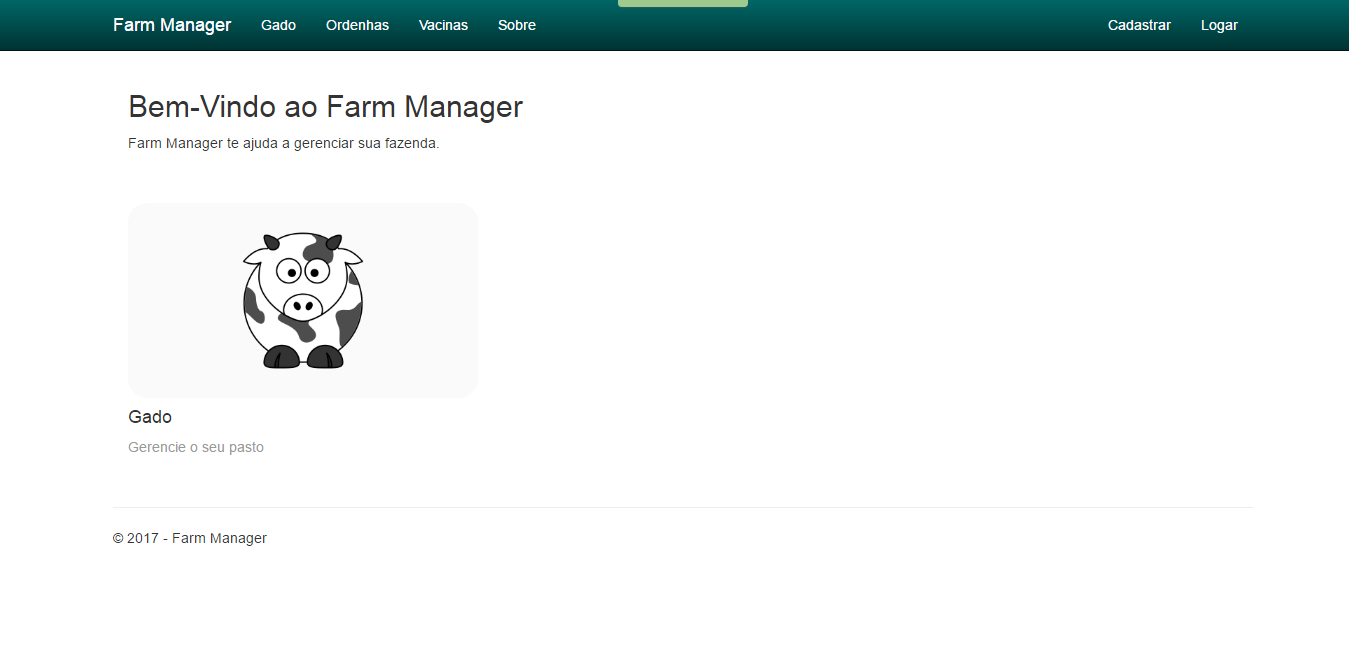
\includegraphics[keepaspectratio=true,scale= 0.5]{figuras/Home-FarmManager.png}
	\caption{Tela Inicial}
	\label{tela-inicial}
\end{figure}
\end{landscape}

A Figura \ref{tela-de-login} apresenta a tela de login da aplicação. O usuário já cadastrado pode então realizar a sua devida autenticação.

\begin{landscape}
\begin{figure}[h!]
	\centering
	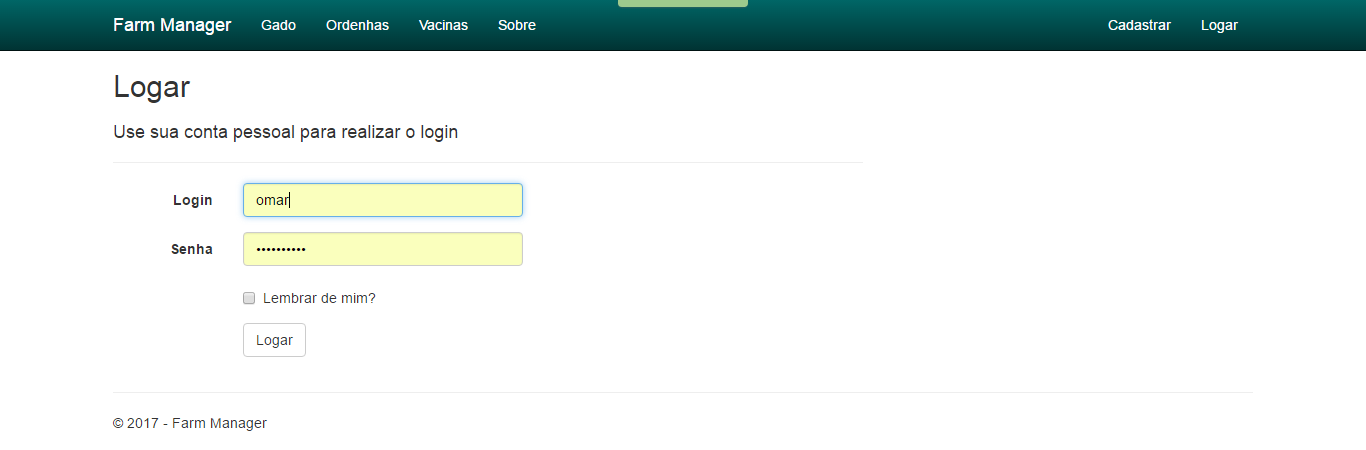
\includegraphics[keepaspectratio=true,scale= 0.7]{figuras/Login-FarmManager.PNG}
	\caption{Tela de Login}
	\label{tela-de-login}
\end{figure}
\end{landscape}

A Figura \ref{tela-de-gado} apresenta a lista de gados registrados na fazenda com suas devidas informações. Nessa tela há a opção de cadastrar um novo gado.

\begin{landscape}
\begin{figure}[h!]
	\centering
	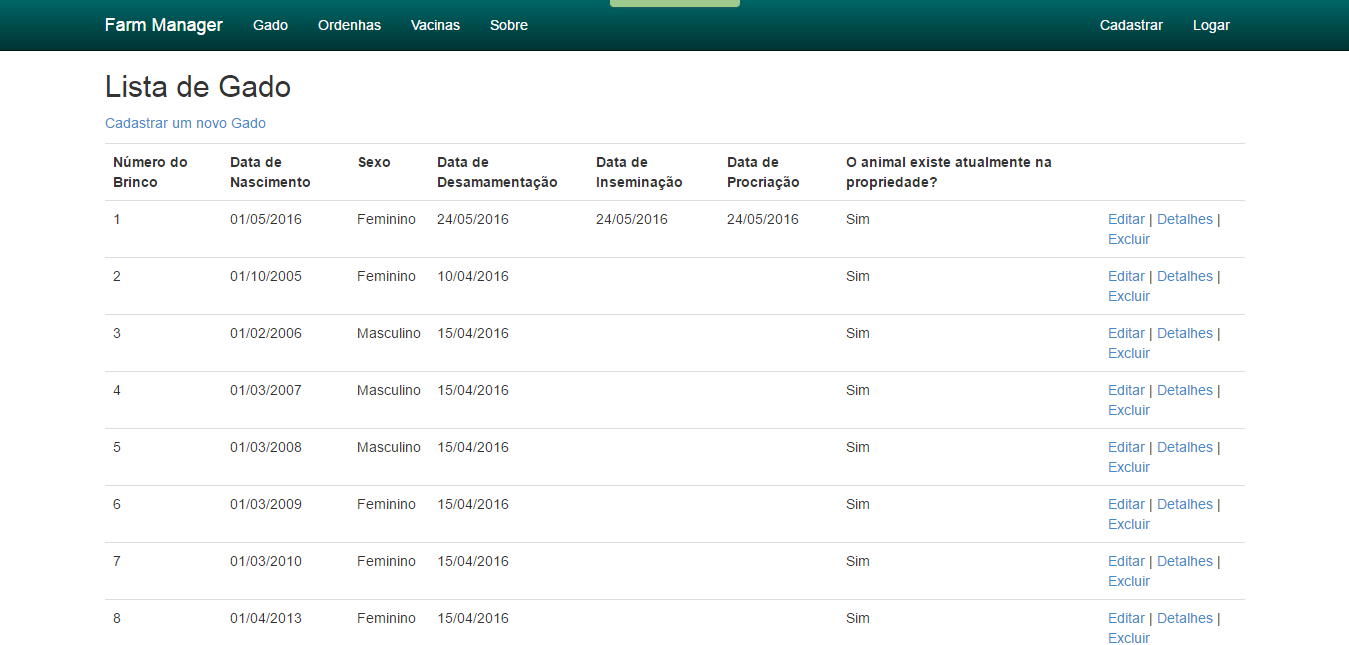
\includegraphics[keepaspectratio=true,scale= 0.5]{figuras/Index-FarmManager.png}
	\caption{Tela de Gado}
	\label{tela-de-gado}
\end{figure}
\end{landscape}

A Figura \ref{tela-de-ordenha} apresenta a lista de ordenhas realizadas na fazenda com suas devidas informações. Nessa tela há a opção de registrar uma nova ordenha.

\begin{landscape}
\begin{figure}[h!]
	\centering
	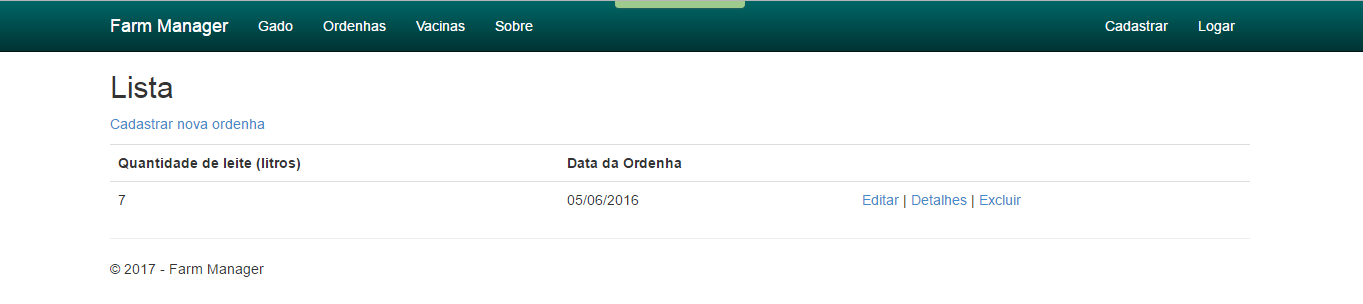
\includegraphics[keepaspectratio=true,scale= 0.7]{figuras/Ordenha-FarmManager.PNG}
	\caption{Tela de Ordenhas}
	\label{tela-de-ordenha}
\end{figure}
\end{landscape}

A Figura \ref{tela-de-vacina} apresenta a lista de vacinas aplicadas nos anivamis da fazenda com suas devidas informações. Nessa tela há a opção de registrar uma nova aplicação de vacina.

\begin{landscape}
\begin{figure}[h!]
	\centering
	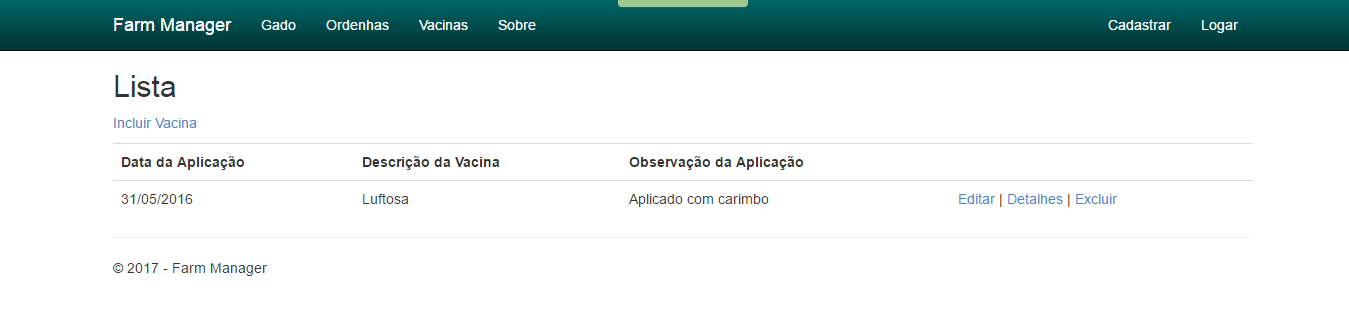
\includegraphics[keepaspectratio=true,scale= 0.5]{figuras/Vacina-FarmManager.png}
	\caption{Tela de Vacinas}
	\label{tela-de-vacina}
\end{figure}
\end{landscape}

Essas são algumas das telas presentes no \textit{software} FarmManager. Não foram apresentadas todas pois é uma grande quantidade e o objetivo dessa subseção era apenas explicitar a interface da aplicação.

\section{Objetivos, Premissas e Restrições}

O objetivo deste projeto é que o projeto FarmManager passe a dar maior ênfase na implantação do produto, através de uma melhoria de processo. Os objetivos a serem atingidos durante a melhoria são:

\begin{itemize}
	\item Elaborar um processo visando uma maior preocupação com o produto final;
	\item Estabelecer o produto para otimização do processo produtivo da fazenda, gerando assim maiores lucros;
	\item Analisar um ponto ideal de frequência para implantações. Conforme dito em apresentação, existe uma linha onde a frequência de implantações passa a precisar de muito esforço apresentando pouco resultado, e outra linha onde o esforço é em vão pois as funcionalidades nunca são entregues para o cliente. Temos como objetivo então encontrar o equilíbrio entre estes dois pontos.
\end{itemize}

Segue conforme a Tabela \ref{premissas-do-projeto}, algumas premissas que servirão de guia para o projeto.

\begin{table}[h!]
\centering
\caption{Premissas do Projeto}
\label{premissas-do-projeto}
\begin{tabular}{|l|l|}
\hline
\textbf{ID} & \textbf{Premissa}                                                                                                                                                                                      \\ \hline
1           & \begin{tabular}[c]{@{}l@{}}Todos os recursos planejados devem ser alocados e entregues conforme\\ as datas previamente estabelecidas.\end{tabular}                                                     \\ \hline
2           & \begin{tabular}[c]{@{}l@{}}Os envolvidos no projeto devem contribuir para a melhoria de processos\\ executados na empresa por meio da identificação e comunicação com as\\ outras partes.\end{tabular} \\ \hline
3           & \begin{tabular}[c]{@{}l@{}}Os gerentes do projeto devem estar comprometidos de forma que\\ participem sempre das atividades críticas.\end{tabular}                                                     \\ \hline
\end{tabular}
\end{table}

\section{Produtos Relevantes}

Os produtos de maior relevância para este projeto serão aqui listados, bem como os responsáveis por seu monitoramento e controle, seu acesso, acesso e de estratégias de segurança relacionados a tais dados. A Tabela \ref{produtos-relevantes} aborda todos estes aspectos.

\begin{table}[h!]
\centering
\caption{Produtos Relevantes}
\label{produtos-relevantes}
\begin{tabular}{|l|l|l|l|l|}
\hline
\textbf{Produto}                                                    & \textbf{\begin{tabular}[c]{@{}l@{}}Responsável pela\\ Coleta\end{tabular}} & \textbf{Meio de Acesso}                                                       & \textbf{Colaboradores}                                                          & \textbf{Tipo de Acesso} \\ \hline
\begin{tabular}[c]{@{}l@{}}Plano de\\ Projeto\\ de MPS\end{tabular} & Equipe de MPS                                                              & \begin{tabular}[c]{@{}l@{}}Compartilhamento\\ online de arquivos\end{tabular} & \begin{tabular}[c]{@{}l@{}}Gerente de\\ Projeto\end{tabular}                    & Leitura                 \\ \hline
Software                                                            & \begin{tabular}[c]{@{}l@{}}Equipe de\\ Desenvolvimento\end{tabular}        & Repositório                                                                   & Equipe Técnica                                                                  & Leitura e Escrita       \\ \hline
Cronograma                                                          & Equipe de MPS                                                              & \begin{tabular}[c]{@{}l@{}}Compartilhamento\\ online de arquivos\end{tabular} & Gerente Sênior                                                                  & Leitura                 \\ \hline
\begin{tabular}[c]{@{}l@{}}Plano de\\ Riscos\end{tabular}           & Equipe de MPS                                                              & \begin{tabular}[c]{@{}l@{}}Compartilhamento\\ online de arquivos\end{tabular} & \begin{tabular}[c]{@{}l@{}}Gerente Sênior\\ e Gerente de\\ Projeto\end{tabular} & Leitura e Escrita       \\ \hline
\end{tabular}
\end{table}